\documentclass[11pt]{standalone}

\usepackage{ifthen}
\usepackage{tikz} 
\usetikzlibrary{shapes.misc}
\usetikzlibrary{arrows,arrows.meta}
\usetikzlibrary{calc,intersections, patterns, math}

\definecolor{pfeil}{RGB}{168,167,167}
\definecolor{petrol}{RGB}{0, 118, 136}
\definecolor{darkgoldenrod}{RGB}{184, 134, 11}
\colorlet{petrol-lighter}{petrol!40}
\colorlet{darkgoldenrod-lighter}{darkgoldenrod!40}

\begin{document}

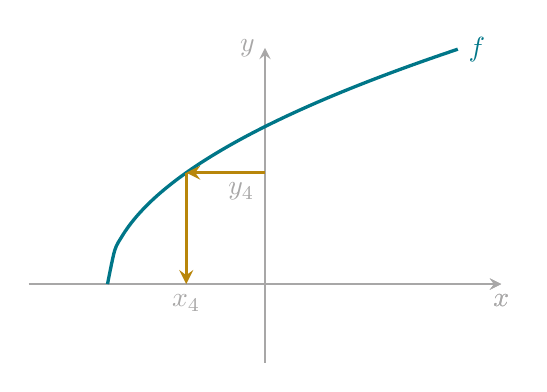
\begin{tikzpicture}[pfeil, scale=2]

    % \draw[thick, fill=petrol!20, draw=petrol-lighter, rounded corners=2ex, opacity=0.5] (0,0) rectangle ++ (1.5,3.5);
    % \draw[thick, fill=darkgoldenrod!20, draw=darkgoldenrod-lighter, rounded corners=2ex, opacity=0.5] (5,0) rectangle ++ (1.5,3.5);

    \draw[thick, -stealth] (-1.5,0) -- (1.5,0) node[below] {$x$};
	\draw[thick, -stealth] (-1.5,0) -- (1.5,0) node[below] {$x$};
	\draw[thick, -stealth] (0,-0.5) -- (0,1.5) node[left] {$y$};
	\draw[very thick, petrol, domain=-1:1.225, smooth, samples=50] plot(\x,{sqrt(\x+1)}) node[right] {$f$};
	\draw[thick] (0,0.707) -- ++ (-0.15,0) node[below] {$y_4$};
	\draw[very thick, -stealth, darkgoldenrod] (0,0.707) -- (-0.5,0.707); 
	\draw[very thick, -stealth, darkgoldenrod] (-0.5,0.707) -- (-0.5,0) node[below, pfeil] {$x_4$};

\end{tikzpicture}

\end{document}
